% Simple CMOS (N-MOSFET & P-MOSFET) H bridge.
% Author: Uli Koehler (https://techoverflow.net)
% Based on http://texample.net/tikz/examples/power-electronics-converter-inverter/
%   by Ali Mehrizi-Sani
%
% NOTE: Requires recent CircuiTikZ version in order to use [T]elmech and fetbodydiode!
% TeXLive 2015 is too old, please use at least TeXLive 2016!

\documentclass[tikz, border=1mm]{standalone}
\usepackage{siunitx}
\usepackage[european,cuteinductors]{circuitikz}

\usetikzlibrary{calc}
\ctikzset{bipoles/thickness=1}
\ctikzset{bipoles/length=0.8cm}
\tikzstyle{every node}=[font=\small]
\tikzstyle{every path}=[line width=0.8pt,line cap=round,line join=round]

\begin{document}
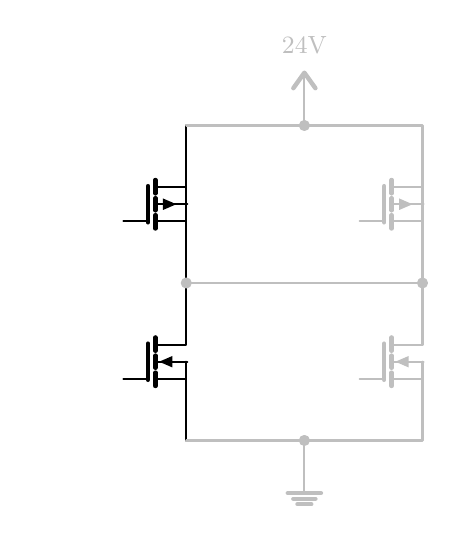
\begin{tikzpicture}
    % Define named coordinates
    \draw (0,0)++(0,4) coordinate (Vcc)
    ++(2,0) coordinate (NE)
    ++(0,-4) coordinate (SE);

    % VCC connection
    \draw[lightgray] (NE)++(1.5,0) to[short,*-,color=lightgray]
    ++(0,0.25) node[color=lightgray,vcc]{24V}

    % GND connection
    (SE)++(1.5,0) to[short,*-,color=lightgray]
    ++(0,-0.25) node[color=lightgray,ground]{}

    % Switches and diodes for left leg
    (NE)++(0,-1) node [color=black,pigfete,scale=0.8,yscale=-1,name=fet1] {}
    ++(0,-2) node [color=black,nigfete,scale=0.8,name=fet4] {};

    \draw [black] (NE) -| (fet1.S)
    (fet1.D) to (fet4.D)
    (fet4.S) |- (SE);

    % Switches and diodes for leg b
    \draw (NE)++(3,0)
    ++(0,-1) node [color=lightgray,pigfete,scale=0.8,yscale=-1,name=fet3] {}
    ++(0,-2) node [color=lightgray,nigfete,scale=0.8,name=fet2] {};
    % --Switch connections for leg b
    \draw[lightgray](NE) -| (fet3.S)
    (fet3.D) -- (fet2.D)
    (fet2.S) |- (SE);

    % Motor (between the legs)
    \draw[draw=lightgray,lightgray] (2,2) to[short,*-*,color=lightgray,current/distance=0.9] ++(3,0)
    ;
\end{tikzpicture}
\end{document}